\section{Resultados}


\subsection{Entrenando la última capa}

\subsubsection{ResNet-50}

\begin{figure}[H]
  \centering
  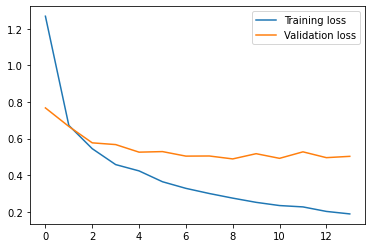
\includegraphics[width=0.5\linewidth]{Imagenes/entrenamiento_redes/ult/resnet_ult_loss.png}
  \caption{Perdida en ResNet50 entrenando unicamente la última capa.}
\end{figure}

\begin{figure}[H]
  \centering
  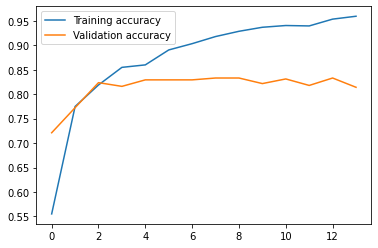
\includegraphics[width=0.5\linewidth]{Imagenes/entrenamiento_redes/ult/resnet_ult_acc.png}
  \caption{Precisión en ResNet50 entrenando unicamente la última capa.}
\end{figure}

\begin{figure}[H]
  \centering
  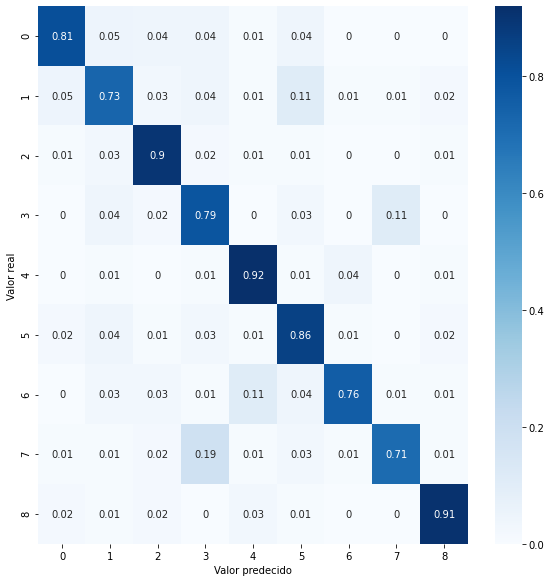
\includegraphics[width=0.5\linewidth]{Imagenes/entrenamiento_redes/ult/resnet_ult_matriz.png}
  \caption{Matriz de confusión sobre los datos de test en ResNet50 entrenando unicamente la última capa.}
\end{figure}

\begin{lstlisting}
Accuracy con ResNet50 entrenando solo ultima capa: 0.8180439727065959
\end{lstlisting}

Vemos que si entrenamos solamente la última capa de ResNet-50, congelando el resto de pesos, obtenemos una Accuracy cercana al 82$%$. Las curvas mostradas en la \textbf{Figura 16} nos dan a entender que el modelo produce un poco de overfitting y que una posible mejora puede ser aplicar técnicas de regularización al mismo. Vamos a ver qué pasa si después de entrenar la última capa, realizamos un ajuste fino de toda la red descongelando los pesos de la misma.

\begin{figure}[H]
  \centering
  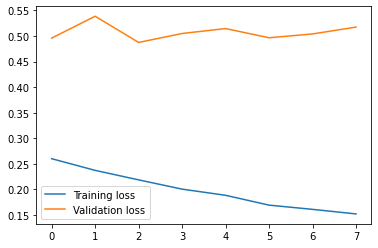
\includegraphics[width=0.5\linewidth]{Imagenes/entrenamiento_redes/ult/resnet_fine_loss.png}
  \caption{Perdida en ResNet50 entrenando unicamente la última capa y tras ajuste fino.}
\end{figure}

\begin{figure}[H]
  \centering
  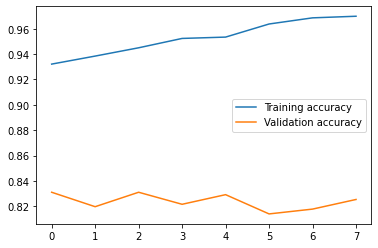
\includegraphics[width=0.5\linewidth]{Imagenes/entrenamiento_redes/ult/resnet_fine_acc.png}
  \caption{Precisión en ResNet50 entrenando unicamente la última capa y tras ajuste fino.}
\end{figure}

\begin{figure}[H]
  \centering
  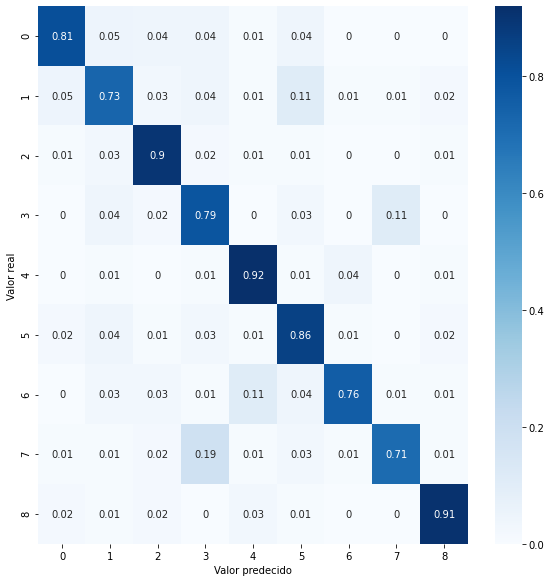
\includegraphics[width=0.5\linewidth]{Imagenes/entrenamiento_redes/ult/resnet_fine_matriz.png}
  \caption{Matriz de confusión sobre los datos de test en ResNet50 entrenando unicamente la última capa y tras ajuste fino..}
\end{figure}

\begin{lstlisting}
Accuracy con ResNet50 tras ajuste fino: 0.8180439727065959
\end{lstlisting}

Si observamos las curvas de precisión de la \textbf{Figura 19} podemos ver que al hacer el ajuste fino los resultados no mejoran. Esto lo podemos observar también al ver la Accuracy en Test, ya que es la misma que cuando hemos entrenado solamente la última capa. La Accuracy se ha mantenido porque estamos usando Early-Stopping y hemos mantenido los pesos que teníamos en vez de empeorarlos.

\subsubsection{DenseNet-121}


\begin{figure}[H]
  \centering
  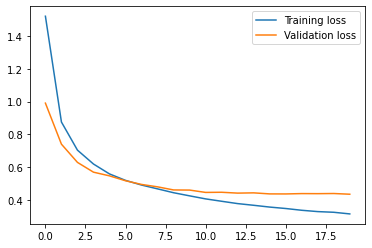
\includegraphics[width=0.5\linewidth]{Imagenes/entrenamiento_redes/ult/densenet_ult_loss.png}
  \caption{Perdida en DenseNet121 entrenando unicamente la última capa.}
\end{figure}

\begin{figure}[H]
  \centering
  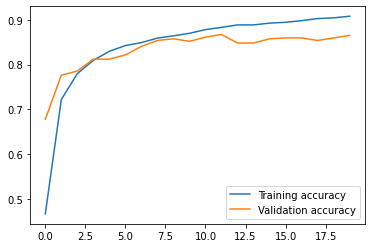
\includegraphics[width=0.5\linewidth]{Imagenes/entrenamiento_redes/ult/densenet_ult_acc.png}
  \caption{Precisión en DenseNet121 entrenando unicamente la última capa.}
\end{figure}

\begin{figure}[H]
  \centering
  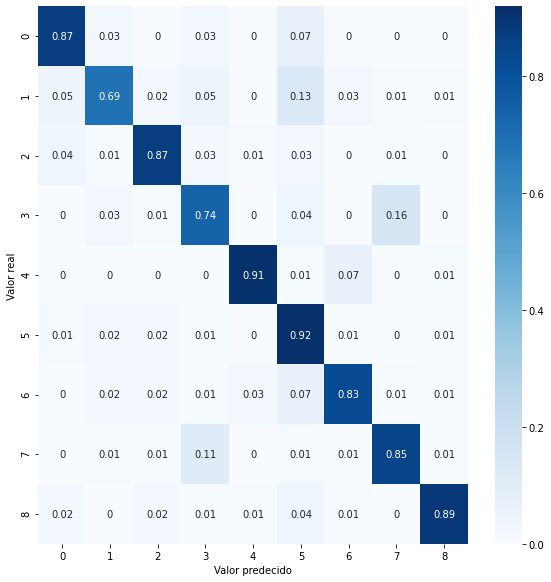
\includegraphics[width=0.5\linewidth]{Imagenes/entrenamiento_redes/ult/densenet_ult_matriz.png}
  \caption{Matriz de confusión sobre los datos de test en DenseNet121 entrenando unicamente la última capa.}
\end{figure}

\begin{lstlisting}
Accuracy con DenseNet121 entrenando solo ultima capa: 0.8377558756633814
\end{lstlisting}

Con DenseNet121, a diferencia que con ResNet50, vemos como no encontramos tanto sobreajuste tras las primeras épocas, aunque los valores de precisión en el conjunto de test son muy similares, aunque un poco mejores que en ResNet50. Observamos como de nuevo es capaz de clasificar las clases sin mucho problema, a excepción de un par de casos concretos que comentaremos al final de los resultados.



\begin{figure}[H]
  \centering
  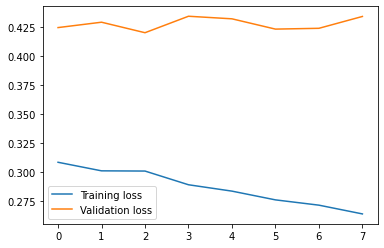
\includegraphics[width=0.5\linewidth]{Imagenes/entrenamiento_redes/ult/densenet_fine_loss.png}
  \caption{Perdida en DenseNet121 entrenando unicamente la última capa y tras ajuste fino.}
\end{figure}

\begin{figure}[H]
  \centering
  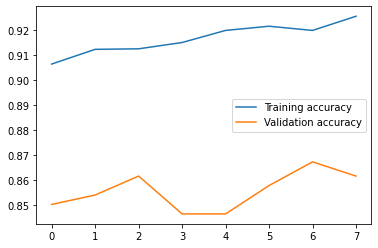
\includegraphics[width=0.5\linewidth]{Imagenes/entrenamiento_redes/ult/densenet_fine_acc.png}
  \caption{Precisión en DenseNet121 entrenando unicamente la última capa y tras ajuste fino.}
\end{figure}

\begin{figure}[H]
  \centering
  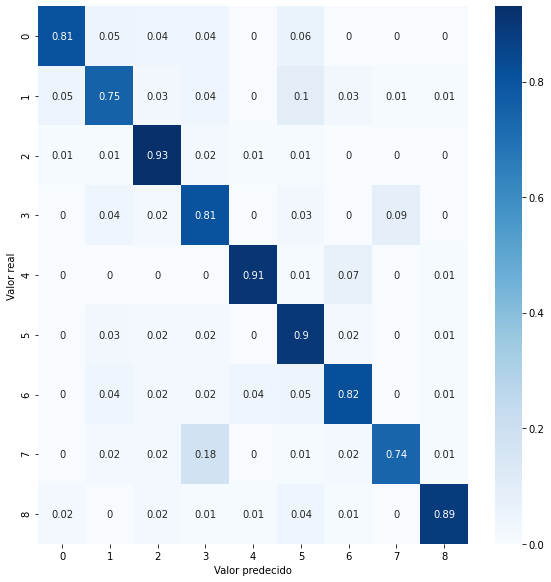
\includegraphics[width=0.5\linewidth]{Imagenes/entrenamiento_redes/ult/densenet_fine_matriz.png}
  \caption{Matriz de confusión sobre los datos de test en DenseNet121 entrenando unicamente la última capa y tras ajuste fino.}
\end{figure}


\begin{lstlisting}
Accuracy con DenseNet121 tras ajuste fino: 0.8385140257771039
\end{lstlisting}

Tras aplicar el fine tuning en DenseNet121 mejora muy levemente, de forma casi imperceptible. Como vemos, en ambos casos se ha obtenido buenos resultados lo que nos da a entender que en DenseNet121 los pesos de ImageNet funcionan bastante bien para nuestro problema.


\subsubsection{InceptionV3}

\begin{figure}[H]
  \centering
  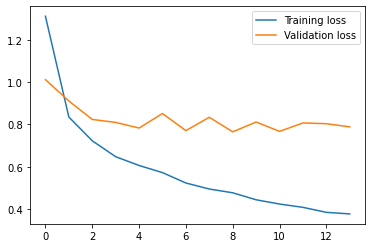
\includegraphics[width=0.5\linewidth]{Imagenes/entrenamiento_redes/ult/inception_ult_loss.png}
  \caption{Perdida en InceptionV3 entrenando unicamente la última capa.}
\end{figure}

\begin{figure}[H]
  \centering
  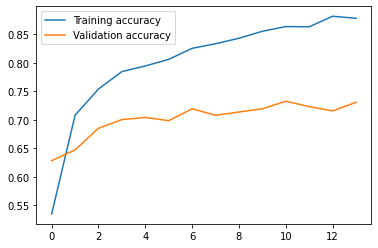
\includegraphics[width=0.5\linewidth]{Imagenes/entrenamiento_redes/ult/inception_ult_acc.png}
  \caption{Precisión en InceptionV3 entrenando unicamente la última capa.}
\end{figure}

\begin{figure}[H]
  \centering
  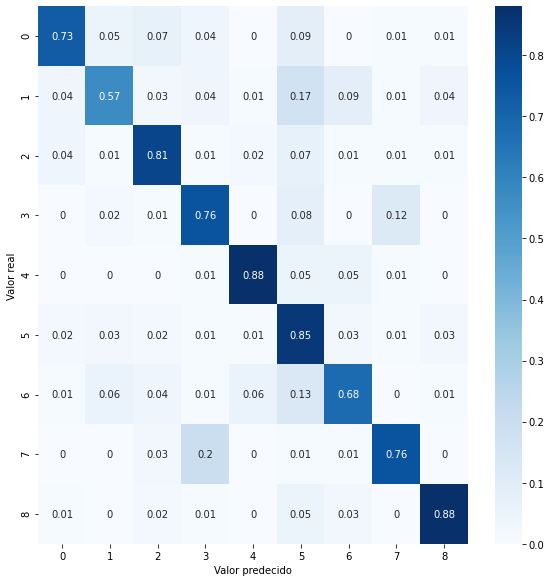
\includegraphics[width=0.5\linewidth]{Imagenes/entrenamiento_redes/ult/inception_ult_matriz.png}
  \caption{Matriz de confusión sobre los datos de test en InceptionV3 entrenando unicamente la última capa.}
\end{figure}


\begin{lstlisting}
Accuracy con InceptionV3 entrenando solo ultima capa: 0.7672479150871873
\end{lstlisting}


\begin{figure}[H]
  \centering
  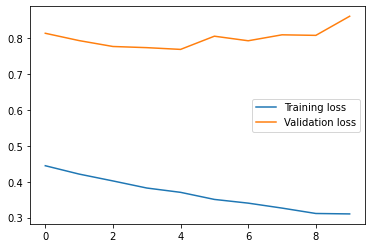
\includegraphics[width=0.5\linewidth]{Imagenes/entrenamiento_redes/ult/inception_fine_loss.png}
  \caption{Perdida en InceptionV3 entrenando unicamente la última capa y tras ajuste fino.}
\end{figure}

\begin{figure}[H]
  \centering
  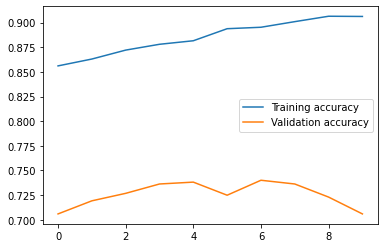
\includegraphics[width=0.5\linewidth]{Imagenes/entrenamiento_redes/ult/inception_fine_acc.png}
  \caption{Precisión en InceptionV3 entrenando unicamente la última capa y tras ajuste fino.}
\end{figure}

\begin{figure}[H]
  \centering
  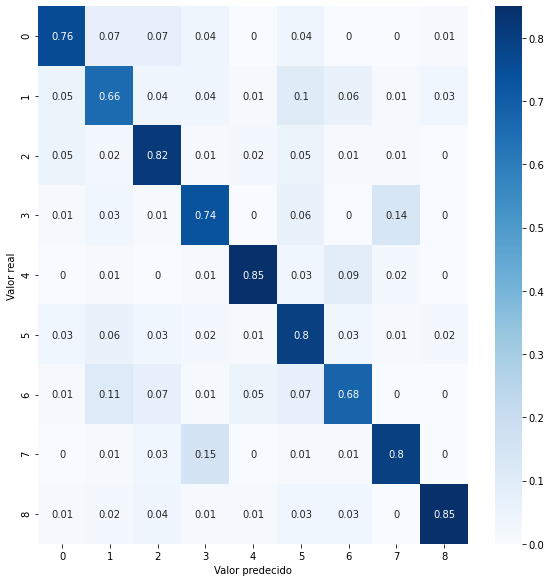
\includegraphics[width=0.5\linewidth]{Imagenes/entrenamiento_redes/ult/inception_fine_matriz.png}
  \caption{Matriz de confusión sobre los datos de test en InceptionV3 entrenando unicamente la última capa y tras ajuste fino.}
\end{figure}


\begin{lstlisting}
Accuracy con InceptionV3 tras ajuste fino: 0.7687642153146323
\end{lstlisting}


\subsubsection{EfficientNetB0}

\begin{figure}[H]
  \centering
  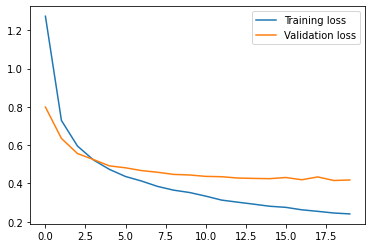
\includegraphics[width=0.5\linewidth]{Imagenes/entrenamiento_redes/ult/efficientnet_ult_loss.png}
  \caption{Perdida en EfficientNetB0 entrenando unicamente la última capa.}
\end{figure}

\begin{figure}[H]
  \centering
  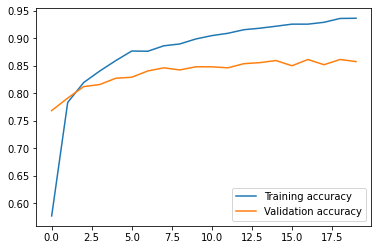
\includegraphics[width=0.5\linewidth]{Imagenes/entrenamiento_redes/ult/efficientnet_ult_acc.png}
  \caption{Precisión en EfficientNetB0 entrenando unicamente la última capa.}
\end{figure}

\begin{figure}[H]
  \centering
  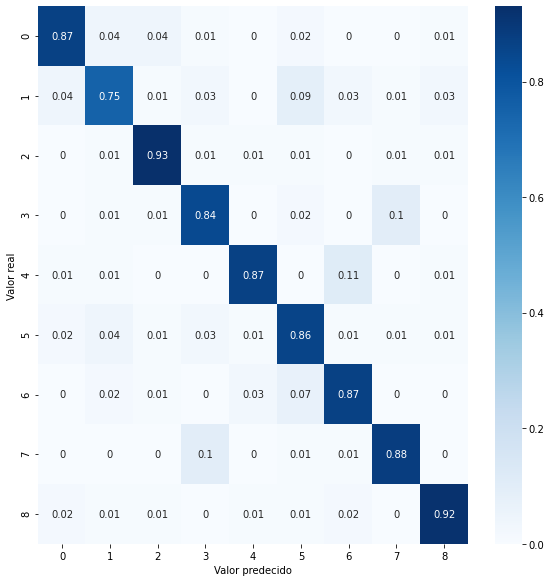
\includegraphics[width=0.5\linewidth]{Imagenes/entrenamiento_redes/ult/efficientnet_ult_matriz.png}
  \caption{Matriz de confusión sobre los datos de test en EfficientNetB0 entrenando unicamente la última capa.}
\end{figure}


\begin{lstlisting}
Accuracy con EfficientNetB0 entrenando solo ultima capa: 0.8612585291887794
\end{lstlisting}

Vemos que EfficientNetB0 comienza con una Accuracy muy alta si observamos las curvas de la \textbf{Figura 34}, llegando hasta un 86$%$ de Accuracy aproximadamente. Es uno de los resultados más altos que hemos obtenido hasta este momento entrenando solamente la capa de salida. Una posible mejora puede ser añadirle regularización a la red para que la curva de validación se mantenga más pegada a la de entrenamiento durante más tiempo. Vamos a ver qué pasa si después de entrenar la última capa, realizamos un ajuste fino de toda la red descongelando los pesos de la misma.


\begin{figure}[H]
  \centering
  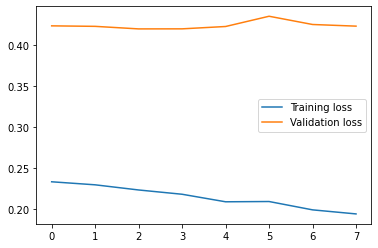
\includegraphics[width=0.5\linewidth]{Imagenes/entrenamiento_redes/ult/efficientnet_fine_loss.png}
  \caption{Perdida en EfficientNetB0 entrenando unicamente la última capa y tras ajuste fino.}
\end{figure}

\begin{figure}[H]
  \centering
  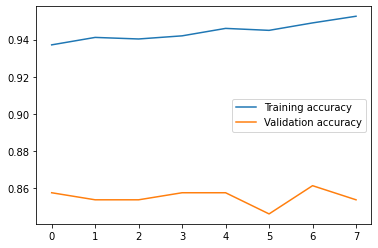
\includegraphics[width=0.5\linewidth]{Imagenes/entrenamiento_redes/ult/efficientnet_fine_acc.png}
  \caption{Precisión en EfficientNetB0 entrenando unicamente la última capa y tras ajuste fino.}
\end{figure}

\begin{figure}[H]
  \centering
  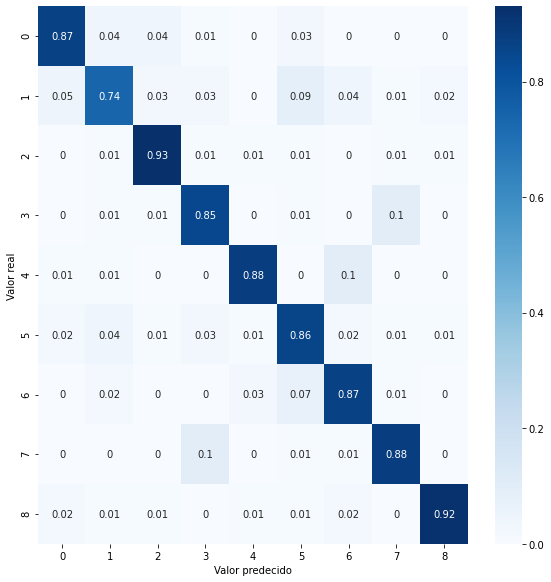
\includegraphics[width=0.5\linewidth]{Imagenes/entrenamiento_redes/ult/efficientnet_fine_matriz.png}
  \caption{Matriz de confusión sobre los datos de test en EfficientNetB0 entrenando unicamente la última capa y tras ajuste fino.}
\end{figure}

\begin{lstlisting}
Accuracy con EfficientNetB0 tras ajuste fino: 0.8627748294162244
\end{lstlisting}



Vemos que al realizar el ajuste fino pasamos de un 86.12$%$ a un 86.27$%$. No se trata de un cambio apreciable como tal pero vamos que los pesos se han ajustado un poco mejor a los datos de nuestro dataset.




% 5ult



\subsection{Entrenando las últimas cinco capas y añadiendo nuevas}

\subsubsection{ResNet-50}

\begin{figure}[H]
  \centering
  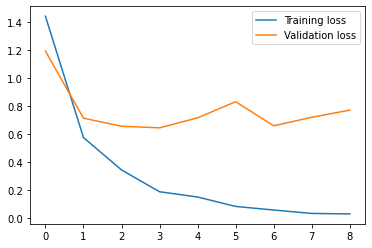
\includegraphics[width=0.5\linewidth]{Imagenes/entrenamiento_redes/5-ult/resnet_5ult_loss.png}
  \caption{Perdida en ResNet50 entrenando las cinco últimas capas y nuevas capas.}
\end{figure}

\begin{figure}[H]
  \centering
  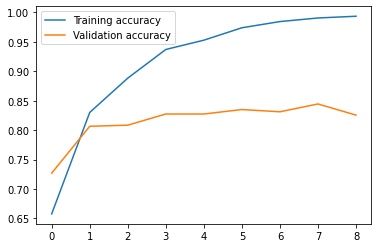
\includegraphics[width=0.5\linewidth]{Imagenes/entrenamiento_redes/5-ult/resnet_5ult_acc.png}
  \caption{Precisión en ResNet50 entrenando las cinco últimas capas y nuevas capas.}
\end{figure}

\begin{figure}[H]
  \centering
  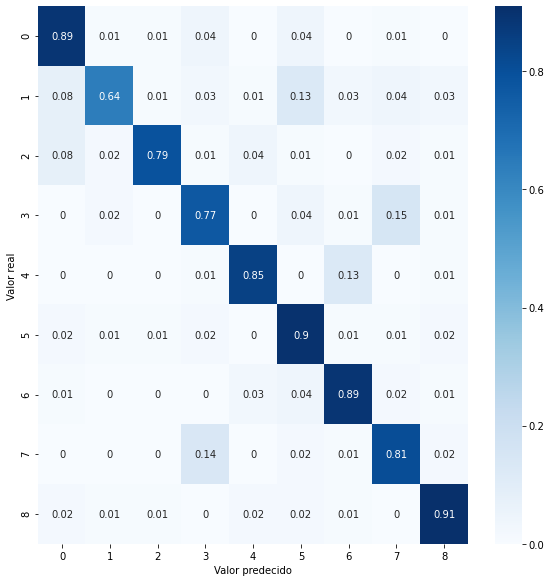
\includegraphics[width=0.5\linewidth]{Imagenes/entrenamiento_redes/5-ult/resnet_5ult_matriz.png}
  \caption{Matriz de confusión sobre los datos de test en ResNet50 entrenando las cinco últimas capas y nuevas capas.}
\end{figure}

\begin{lstlisting}
Accuracy con ResNet50 entrenando las cinco últimas capas: 0.821076573161486
\end{lstlisting}


Al entrenar las cinco últimas capas en vez de solamente la última, y añadir nuevas capas Dense, BatchNormalization y Dropout; obtenemos una accuracy del 82$%$ aproximadamente. Si miramos la Accuracy que obtuvimos cuando solo entrenamos la última capa, podemos apreciar una pequeña mejora. Vamos a ver que pasa si ahora hacemos un ajuste fino con estos nuevos pesos de las últimas capas.

\begin{figure}[H]
  \centering
  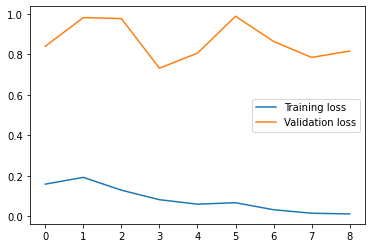
\includegraphics[width=0.5\linewidth]{Imagenes/entrenamiento_redes/5-ult/resnet_5fine_loss.png}
  \caption{Perdida en ResNet50 entrenando las cinco últimas capas y nuevas capas tras ajuste fino.}
\end{figure}

\begin{figure}[H]
  \centering
  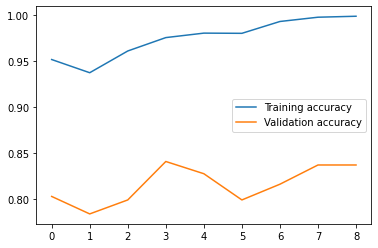
\includegraphics[width=0.5\linewidth]{Imagenes/entrenamiento_redes/5-ult/resnet_5fine_acc.png}
  \caption{Precisión en ResNet50 entrenando las cinco últimas capas y nuevas capas tras ajuste fino.}
\end{figure}

\begin{figure}[H]
  \centering
  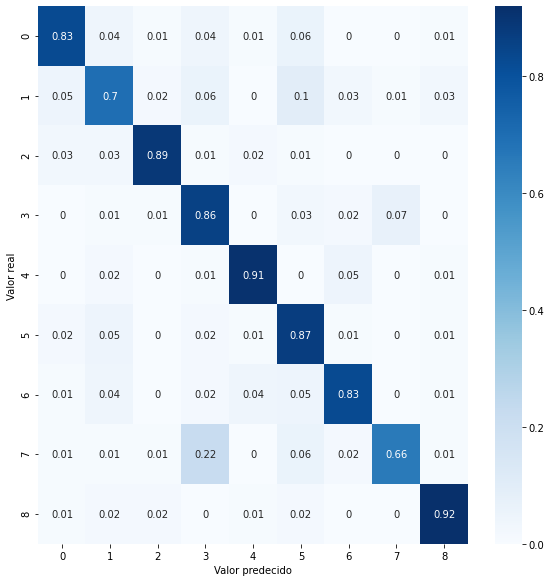
\includegraphics[width=0.5\linewidth]{Imagenes/entrenamiento_redes/5-ult/resnet_5fine_matriz.png}
  \caption{Matriz de confusión sobre los datos de test en ResNet50 entrenando las cinco últimas capas y nuevas capas tras ajuste fino..}
\end{figure}


\begin{lstlisting}
Accuracy con ResNet50 tras ajuste fino: 0.8256254738438211
\end{lstlisting}


Vemos que hemos mejorado un poco más, pasando de un 82.1$%$ a un 82.56$%$. No se trata de una mejora apreciable, como el resto de las mejoras que hemos observado, pero sabemos que estamos yendo por el camino correcto.

\subsubsection{DenseNet-121}

\begin{figure}[H]
  \centering
  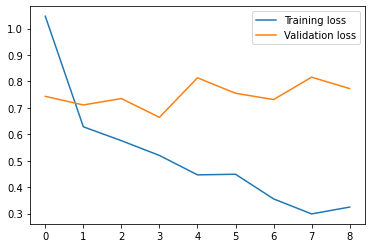
\includegraphics[width=0.5\linewidth]{Imagenes/entrenamiento_redes/5-ult/densenet_5ult_loss.png}
  \caption{Perdida en DenseNet121 entrenando las cinco últimas capas y nuevas capas.}
\end{figure}

\begin{figure}[H]
  \centering
  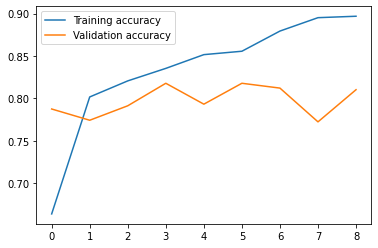
\includegraphics[width=0.5\linewidth]{Imagenes/entrenamiento_redes/5-ult/densenet_5ult_acc.png}
  \caption{Precisión en DenseNet121 entrenando las cinco últimas capas y nuevas capas.}
\end{figure}

\begin{figure}[H]
  \centering
  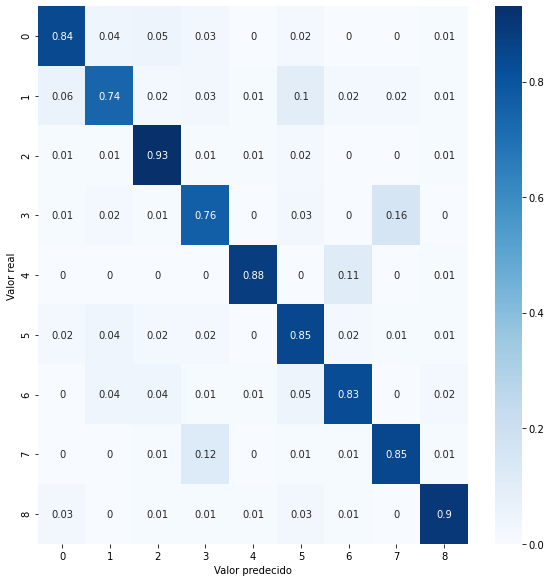
\includegraphics[width=0.5\linewidth]{Imagenes/entrenamiento_redes/5-ult/densenet_5ult_matriz.png}
  \caption{Matriz de confusión sobre los datos de test en DenseNet121 entrenando las cinco últimas capas y nuevas capas.}
\end{figure}


\begin{lstlisting}
Accuracy con DenseNet121 entrenando las ultimas 5 capas: 0.8339651250947687
\end{lstlisting}



\begin{figure}[H]
  \centering
  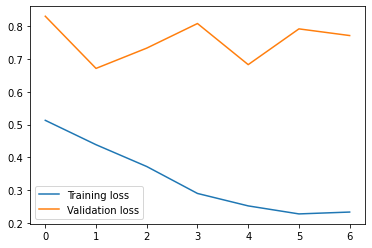
\includegraphics[width=0.5\linewidth]{Imagenes/entrenamiento_redes/5-ult/densenet_5fine_loss.png}
  \caption{Perdida en DenseNet121 entrenando las cinco últimas capas y nuevas capas tras ajuste fino.}
\end{figure}

\begin{figure}[H]
  \centering
  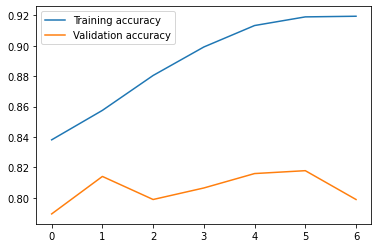
\includegraphics[width=0.5\linewidth]{Imagenes/entrenamiento_redes/5-ult/densenet_5fine_acc.png}
  \caption{Precisión en DenseNet121 entrenando las cinco últimas capas y nuevas capas tras ajuste fino.}
\end{figure}

\begin{figure}[H]
  \centering
  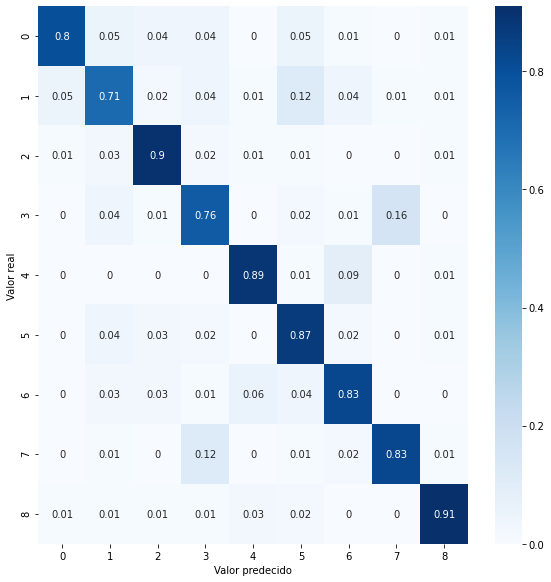
\includegraphics[width=0.5\linewidth]{Imagenes/entrenamiento_redes/5-ult/densenet_5fine_matriz.png}
  \caption{Matriz de confusión sobre los datos de test en DenseNet121 entrenando las cinco últimas capas y nuevas capas tras ajuste fino.}
\end{figure}

\begin{lstlisting}
Accuracy con DenseNet121 tras ajuste fino: 0.8263836239575436
\end{lstlisting}



\subsubsection{InceptionV3}


\begin{figure}[H]
  \centering
  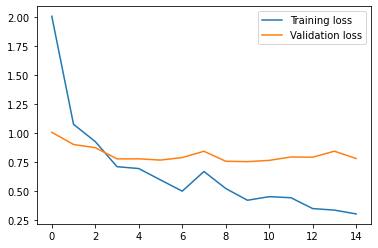
\includegraphics[width=0.5\linewidth]{Imagenes/entrenamiento_redes/5-ult/inception_5ult_loss.png}
  \caption{Perdida en InceptionV3 entrenando las cinco últimas capas y nuevas capas.}
\end{figure}

\begin{figure}[H]
  \centering
  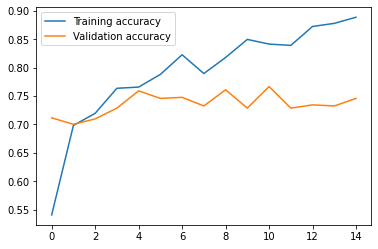
\includegraphics[width=0.5\linewidth]{Imagenes/entrenamiento_redes/5-ult/inception_5ult_acc.png}
  \caption{Precisión en InceptionV3 entrenando las cinco últimas capas y nuevas capas.}
\end{figure}

\begin{figure}[H]
  \centering
  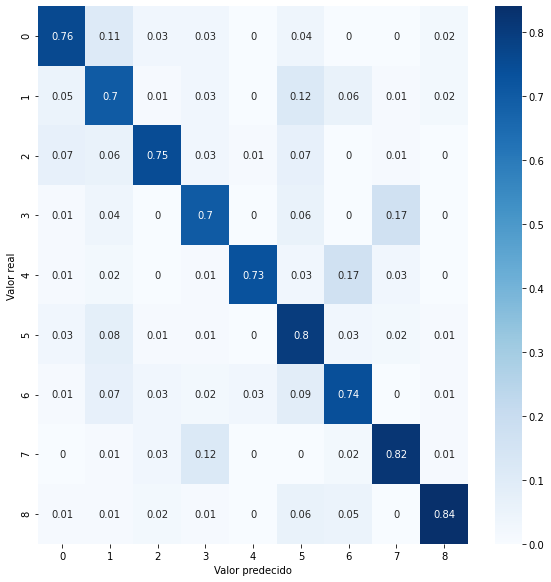
\includegraphics[width=0.5\linewidth]{Imagenes/entrenamiento_redes/5-ult/inception_5ult_matriz.png}
  \caption{Matriz de confusión sobre los datos de test en InceptionV3 entrenando las cinco últimas capas y nuevas capas.}
\end{figure}


\begin{lstlisting}
Accuracy con InceptionV3 entrenando las cinco últimas capas: 0.7589082638362395
\end{lstlisting}


\begin{figure}[H]
  \centering
  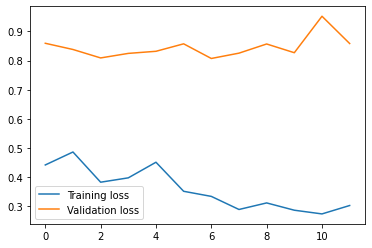
\includegraphics[width=0.5\linewidth]{Imagenes/entrenamiento_redes/5-ult/inception_5fine_loss.png}
  \caption{Perdida en InceptionV3 entrenando las cinco últimas capas y nuevas capas tras ajuste fino.}
\end{figure}

\begin{figure}[H]
  \centering
  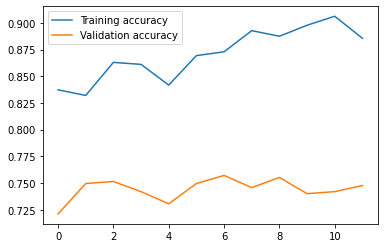
\includegraphics[width=0.5\linewidth]{Imagenes/entrenamiento_redes/5-ult/inception_5fine_acc.png}
  \caption{Precisión en InceptionV3 entrenando las cinco últimas capas y nuevas capas tras ajuste fino.}
\end{figure}

\begin{figure}[H]
  \centering
  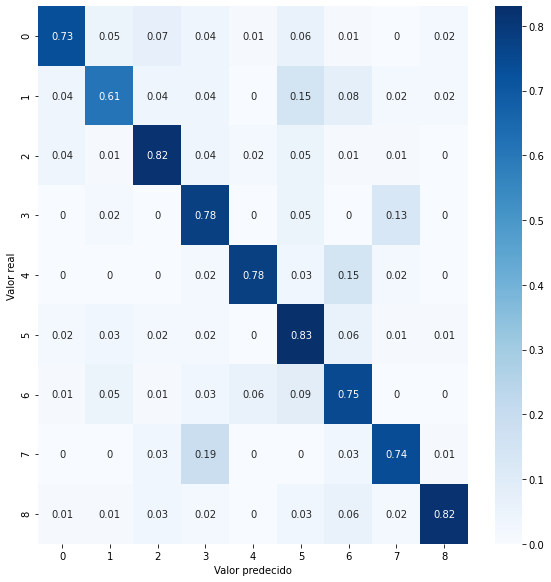
\includegraphics[width=0.5\linewidth]{Imagenes/entrenamiento_redes/5-ult/inception_5fine_matriz.png}
  \caption{Matriz de confusión sobre los datos de test en InceptionV3 entrenando las cinco últimas capas y nuevas capas tras ajuste fino.}
\end{figure}


\begin{lstlisting}
Accuracy con InceptionV3 tras ajuste fino: 0.7649734647460197
\end{lstlisting}



\subsubsection{EfficientNetB0}


\begin{figure}[H]
  \centering
  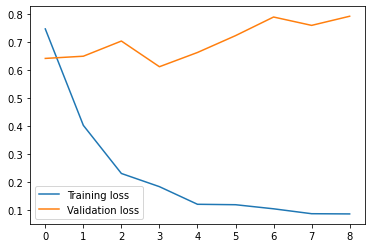
\includegraphics[width=0.5\linewidth]{Imagenes/entrenamiento_redes/5-ult/efficientnet_5ult_loss.png}
  \caption{Perdida en EfficientNetB0 entrenando las cinco últimas capas y nuevas capas.}
\end{figure}

\begin{figure}[H]
  \centering
  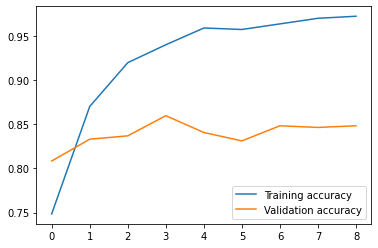
\includegraphics[width=0.5\linewidth]{Imagenes/entrenamiento_redes/5-ult/efficientnet_5ult_acc.png}
  \caption{Precisión en EfficientNetB0 entrenando las cinco últimas capas y nuevas capas.}
\end{figure}

\begin{figure}[H]
  \centering
  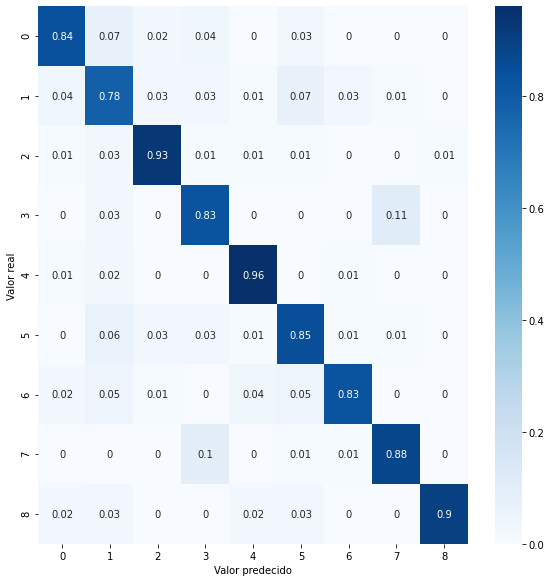
\includegraphics[width=0.5\linewidth]{Imagenes/entrenamiento_redes/5-ult/efficientnet_5ult_matriz.png}
  \caption{Matriz de confusión sobre los datos de test en EfficientNetB0 entrenando las cinco últimas capas y nuevas capas.}
\end{figure}


\begin{lstlisting}
Accuracy con EfficientNetB0 entrenando las cinco últimas capas: 0.8597422289613343
\end{lstlisting}


Al añadir más capas y entrenar las últimas cinco podemos ver que se produce mucho más overfitting que cuando solo entrenamos la última capa (Figuras 34 y 58). Incluso la Accuracy en Test ha bajado de un 86.12$%$ a un 85.9$%$. Esta decisión ha perjudicado un poco el rendimiento de la red EfficientNetB0. Vamos a ver si al realizar Fine Tuning mejoramos o seguimos empeorando.

\begin{figure}[H]
  \centering
  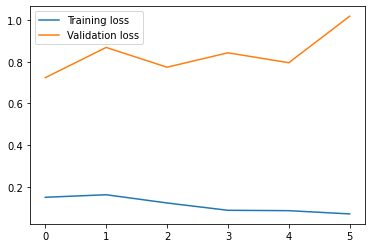
\includegraphics[width=0.5\linewidth]{Imagenes/entrenamiento_redes/5-ult/efficientnet_5fine_loss.png}
  \caption{Perdida en EfficientNetB0 entrenando las cinco últimas capas y nuevas capas tras ajuste fino.}
\end{figure}

\begin{figure}[H]
  \centering
  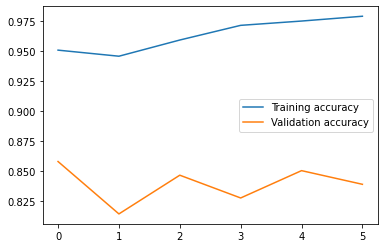
\includegraphics[width=0.5\linewidth]{Imagenes/entrenamiento_redes/5-ult/efficientnet_5fine_acc.png}
  \caption{Precisión en EfficientNetB0 entrenando las cinco últimas capas y nuevas capas tras ajuste fino.}
\end{figure}

\begin{figure}[H]
  \centering
  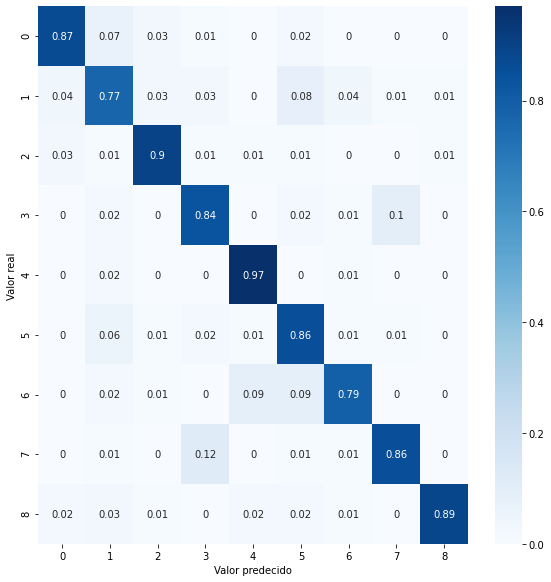
\includegraphics[width=0.5\linewidth]{Imagenes/entrenamiento_redes/5-ult/efficientnet_5fine_matriz.png}
  \caption{Matriz de confusión sobre los datos de test en EfficientNetB0 entrenando las cinco últimas capas y nuevas capas tras ajuste fino.}
\end{figure}


\begin{lstlisting}
Accuracy con EfficientNetB0 tras ajuste fino: 0.8567096285064443
\end{lstlisting}


Como vemos, al realizar Fine Tuning seguimos empeorando, lo que nos lleva a asegurar que las capas elegidas y descongeladas no han sido las más adecuadas para mejorar el rendimiento de la red.